\documentclass[10pt,a4paper]{article}

\usepackage{amsmath}
\usepackage{amsfonts}
\usepackage{amssymb}
\usepackage{graphicx}
\usepackage{float}
\usepackage[polish]{babel}
\usepackage[utf8]{inputenc}
\usepackage{polski}
\frenchspacing

\author{Marcin Ochman}
\title{Algorytmy sortowania: Quick Sort, Merge Sort, Heap Sort - porównanie wydajności. }

\begin{document}
\maketitle
\section{Opis problemu}

Sortowanie to jedna z najczęstszych czynności wykonywana przez obecne komputery.
Ogromne bazy danych, z którymi programiści mają do czynienia wymagają od nich
odpowiedniej wiedzy, jak szybko móc te dane umieścić w określonym porządku.
Sortowanie w świecie algorytmów ma swoje szczególne miejsce. Algorytmy sortowania są
dobrze przeanalizowane, znamy ich złożoności obliczeniowe, zapotrzebowanie na pamięć.
Jednymi z najpopularniejszych są tytułowe:
\begin{itemize}
	\item sortowanie szybkie
	\item sortowanie przez scalanie
	\item sortowanie przez kopcowanie
\end{itemize}
Co ciekawe, wszystkie algorytmy wykorzystują w pewien sposób rekurencję.


\section{Krótki opis algorytmów}

W tej częsci przybliżę pokrótce każdy z algorytmów i postaram się podać jego mocne i
słabe strony.

\subsection{Quick Sort}

Jest to obecnie najczęściej wykorzystywany algorytm sortowania. Średni czas wykonywania
dla określonego rozmiaru problemu w porównaniu do innych algorytmów jest najmniejszy.
Złożoność obliczeniowa w przypadku średnim wynosi $\mathcal{O}(n\log_2 n)$.
Co ciekawe, przy pesymistycznym przypadku tj. dane posortowane odwrotnie, ma
złożoność $\mathcal{O}(n^2)$. Pomimo tego, jest on jednym z najszybszych znanych 
algorytmów sortowania poprzez porównywanie. Dane dzielonę są na dwie części, 
w pierwszej części znajdują się elementy mniejsze od piwota, w drugiej większe. 
Podziału tego dokonujemy poprzez funkcję zwyczajowo nazywaną partition. Następnie
wywołujemy rekurencyjnie funkcję osobno dla dwóch podtablic.

\subsection{Merge Sort}

Koncepcja sortowania przez scalanie jest bardzo prosta. Jeśli mamy już posortowane dwie tablice,
to jedynym problemem jest połączenie je w jedną, dużą tablicę. Należy odpowiednio porównywać
elementy z jednej tablicy i z drugiej, a następnie dodawać do tablicy wynikowej. Pojawia się
pytanie ,,jak otrzymać posortowane już dwie tablice''? Wystarczy scalać tablice o rozmiarze 1.
Algorytm ma złożoność $\mathcal{O}(n\log_2 n )$. Wadą tego algorytmu jest zapotrzebowanie na
dodatkową pamięć.

\subsection{Heap Sort}

Sortowanie przez kopcowanie, jak można się domyślić, wykorzystuje strukturę danych zwaną kopcem.
Kopiec to drzewo binarne, w którym pomiędzy synem a ojcem występuje pewna relacja. Jeśli ojciec jest,
większy od syna jest to kopiec typu maks, jeśli jest odwrotnie jest to kopiec typu min. Algorytm polega
na zbudowaniu kopca, a następnie ściaganiu odpowiednich elementów. Złożoność obliczeniowa to 
$\mathcal{O}(n\log_2 n)$

\section{Wyniki testów wydajnościowych}

Poniżej zostały przedstawione wykresy zależności czasu wykonywania od rozmiaru problemu.
Algorytmy zostały zbadane dla tych samych zbiorów danych. Jedynie w przypadku analizy 
sortowania szybkiego dla przypadku pesymistycznego użyto odrębnego zbioru.

\subsection{Quick Sort - przypadek pesymistyczny}

\begin{figure}[H]
\centering
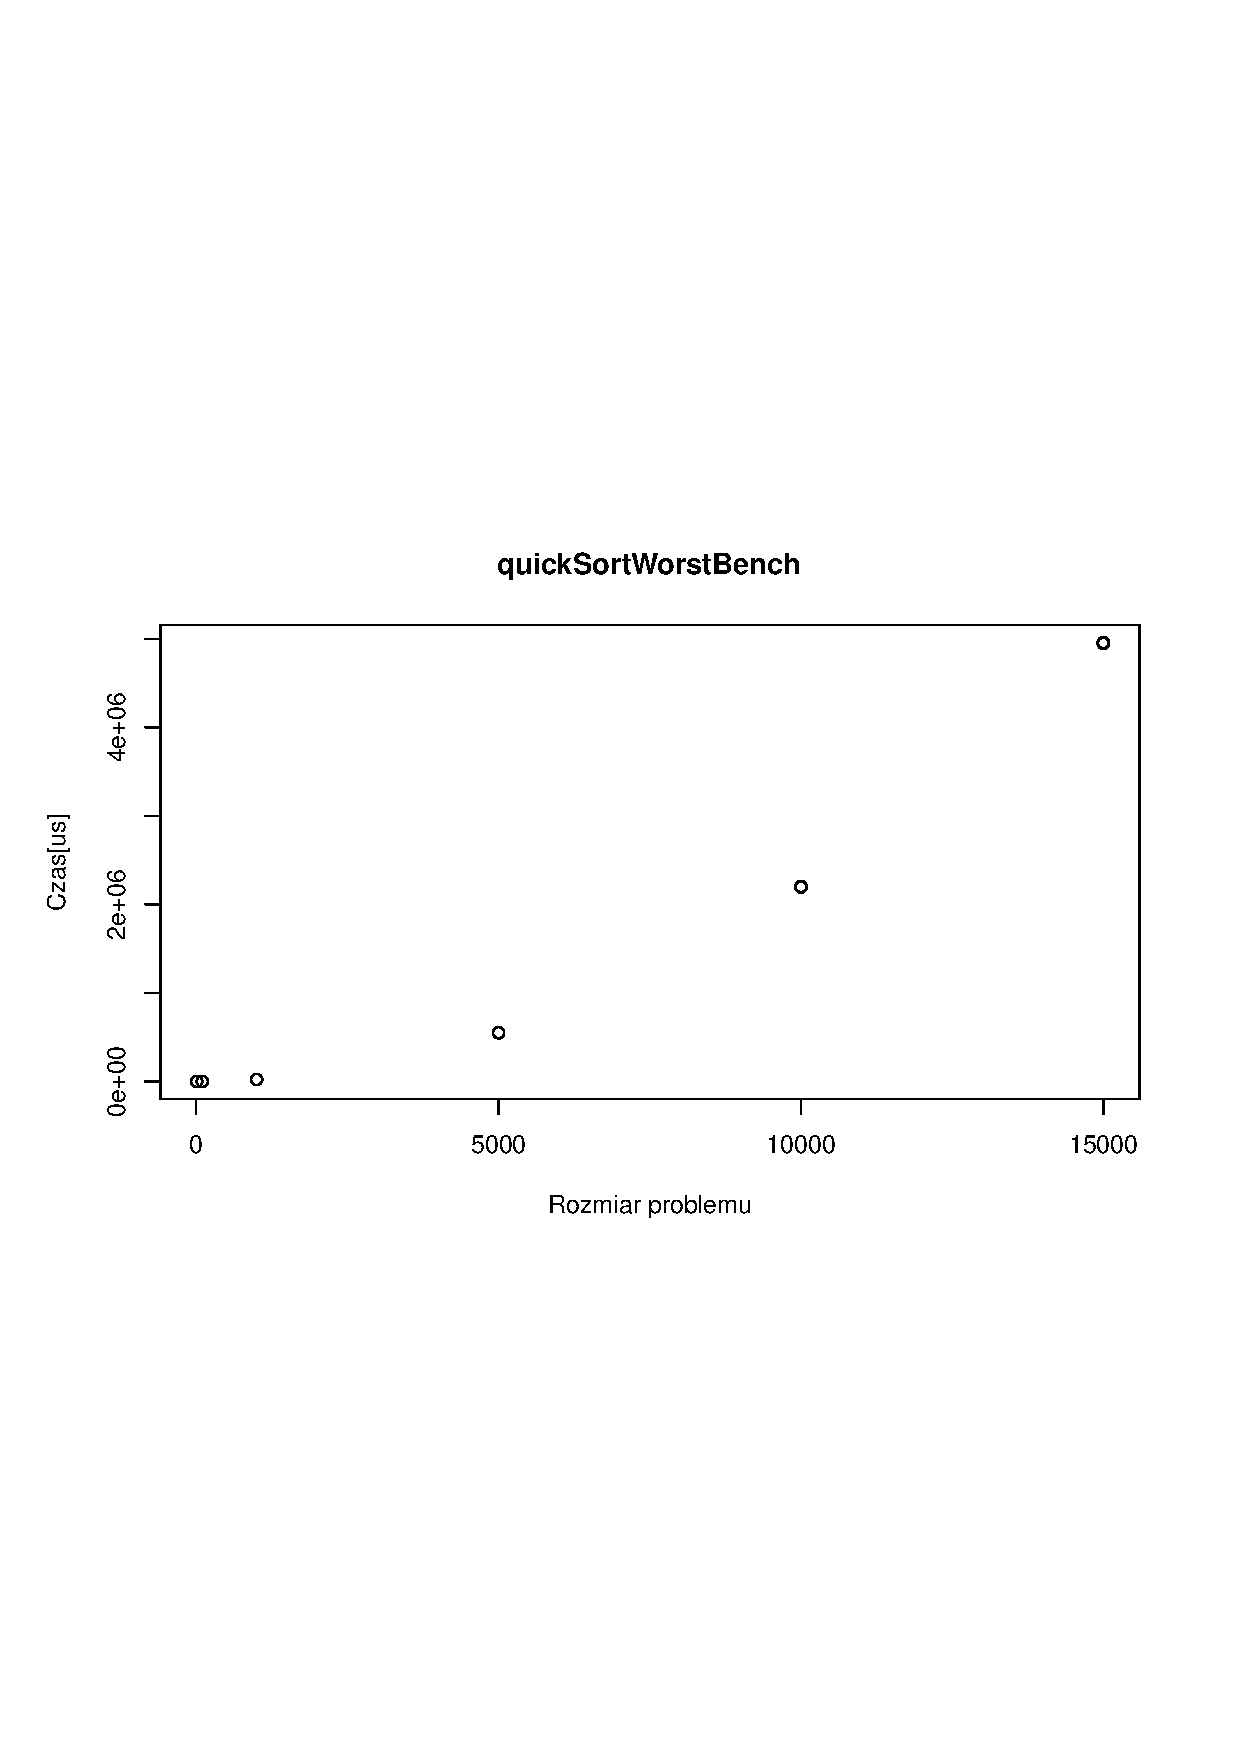
\includegraphics[width=0.7\linewidth]{./Wykresy/quickSortWorstBench}
\caption{Zależność czasu wykonania od rozmiaru problemu - Quick Sort - przypadek pesymistyczny. Kolor czarny - wersja z losowaniem piwotu,
kolor czerwony - piwot na końcu tablicy}
\label{fig:quickSortWorstBench}
\end{figure}
\subsection{Quick Sort - przypadek średni}

\begin{figure}[H]
\centering
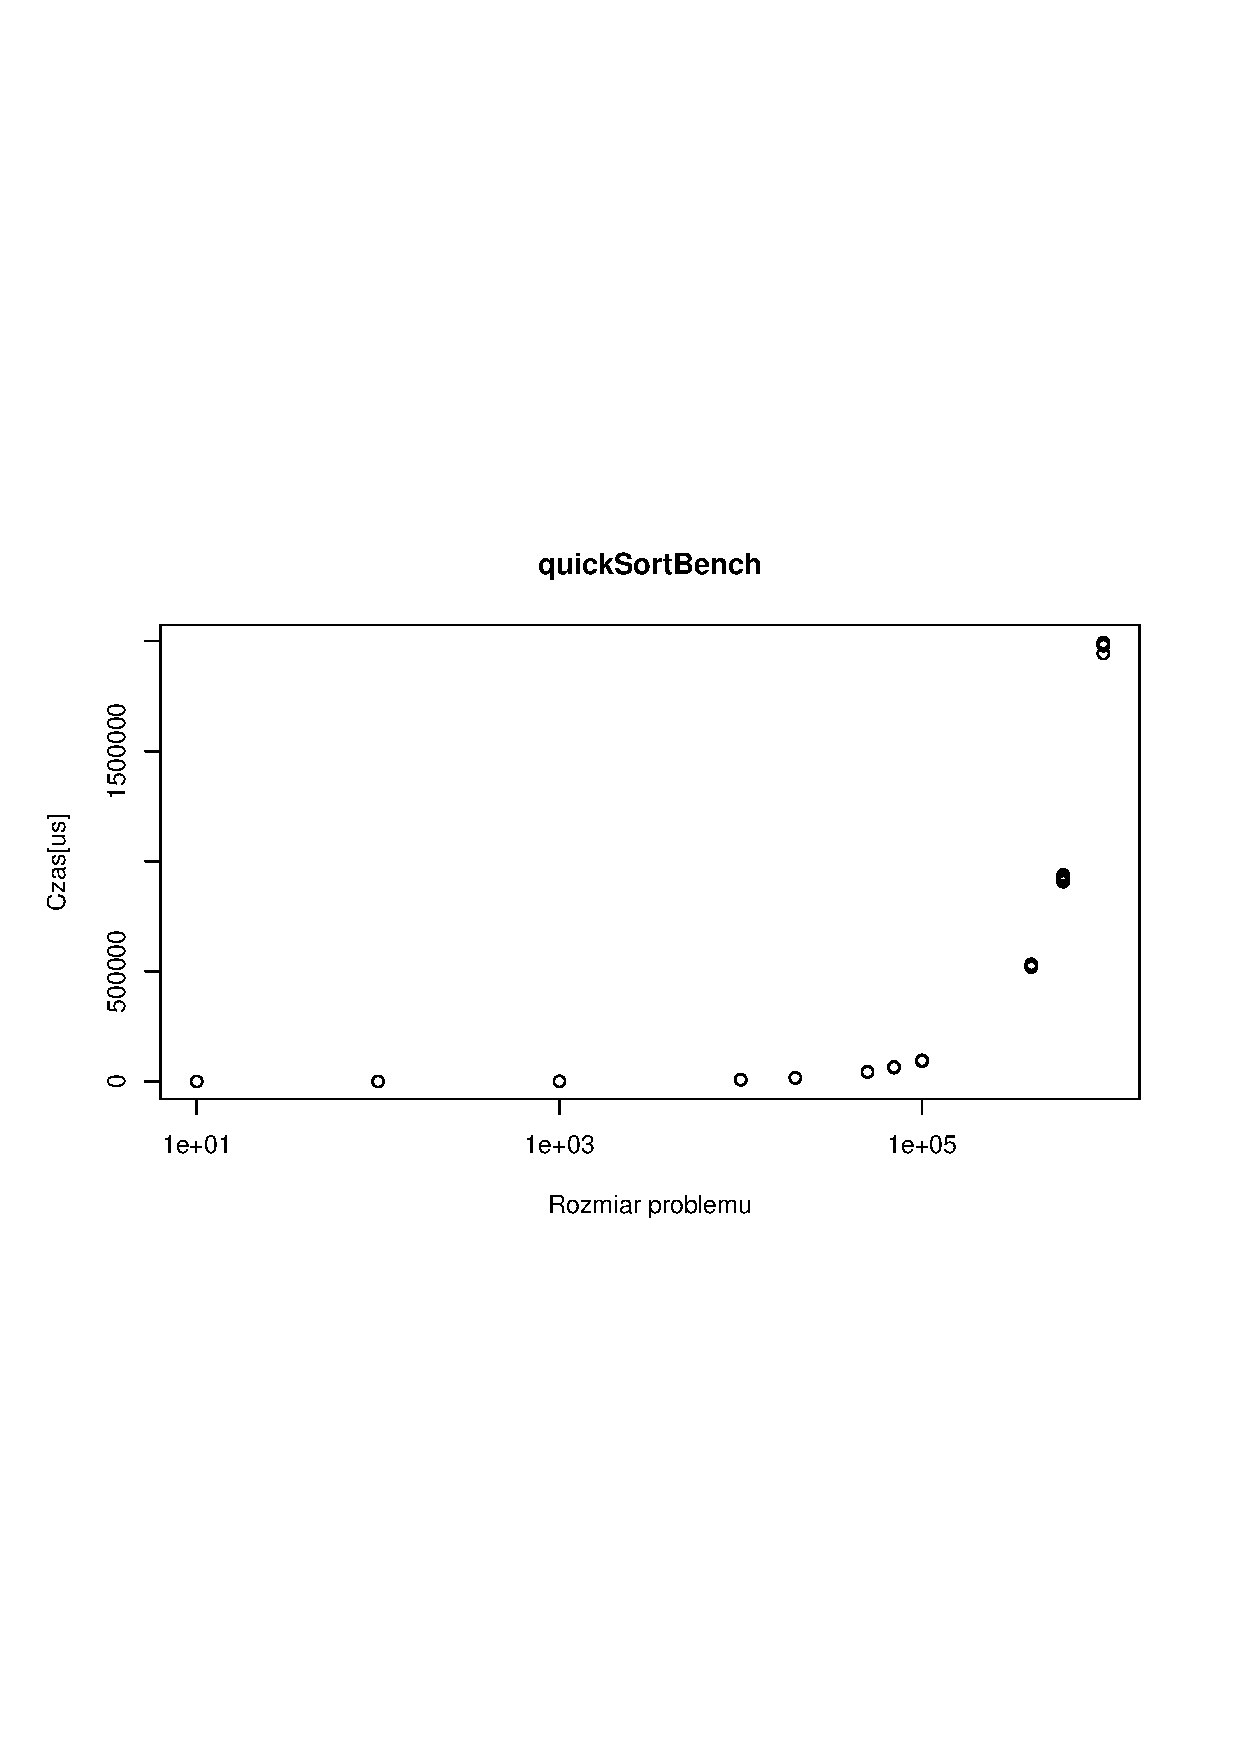
\includegraphics[width=0.7\linewidth]{./Wykresy/quickSortBench}
\caption{Zależność czasu wykonania od rozmiaru problemu - Quick Sort - przypadek średni}
\label{fig:quickSortBench}
\end{figure}

\subsection{Heap Sort}

\begin{figure}[H]
\centering
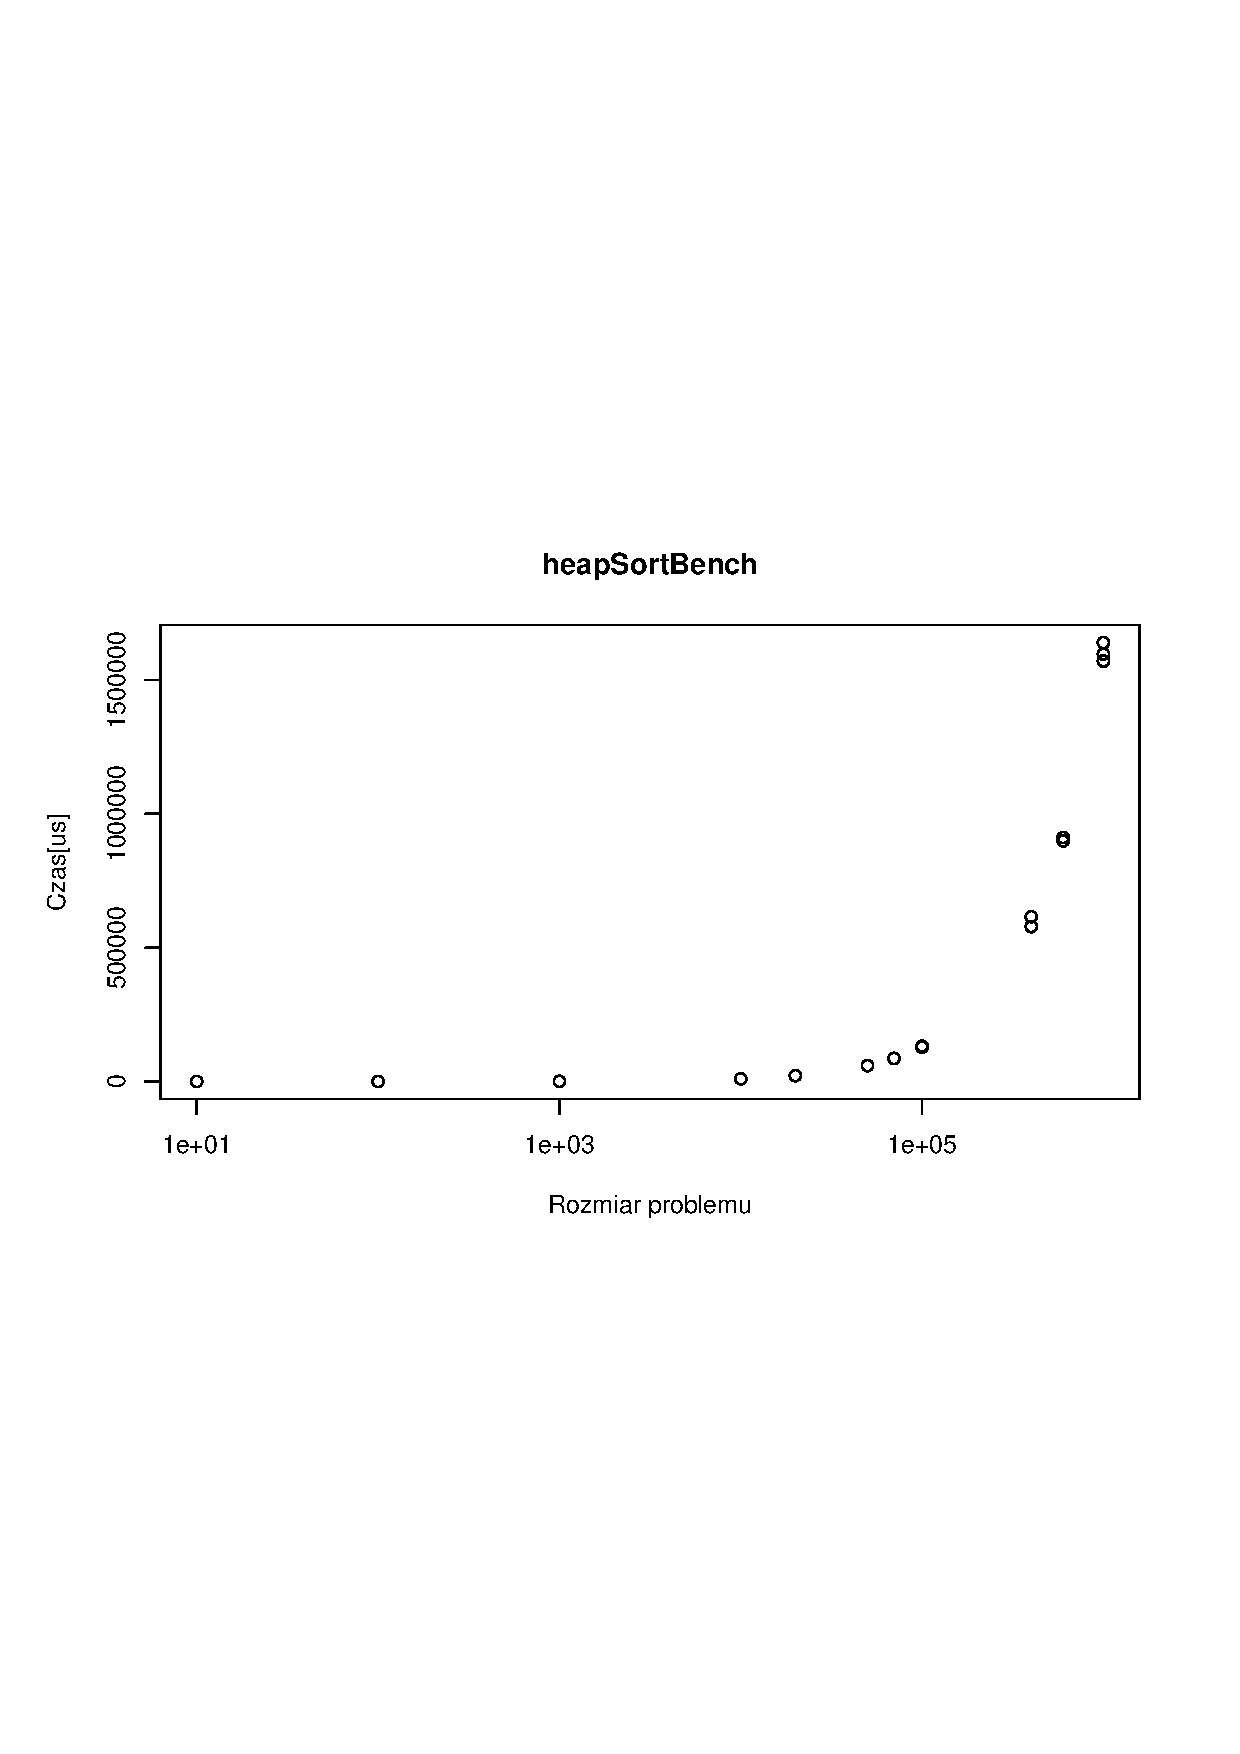
\includegraphics[width=0.7\linewidth]{./Wykresy/heapSortBench}
\caption{Zależność czasu wykonania od rozmiaru problemu - Heap Sort}
\label{fig:heapSortBench}
\end{figure}

\subsection{Merge Sort}

\begin{figure}[H]
\centering
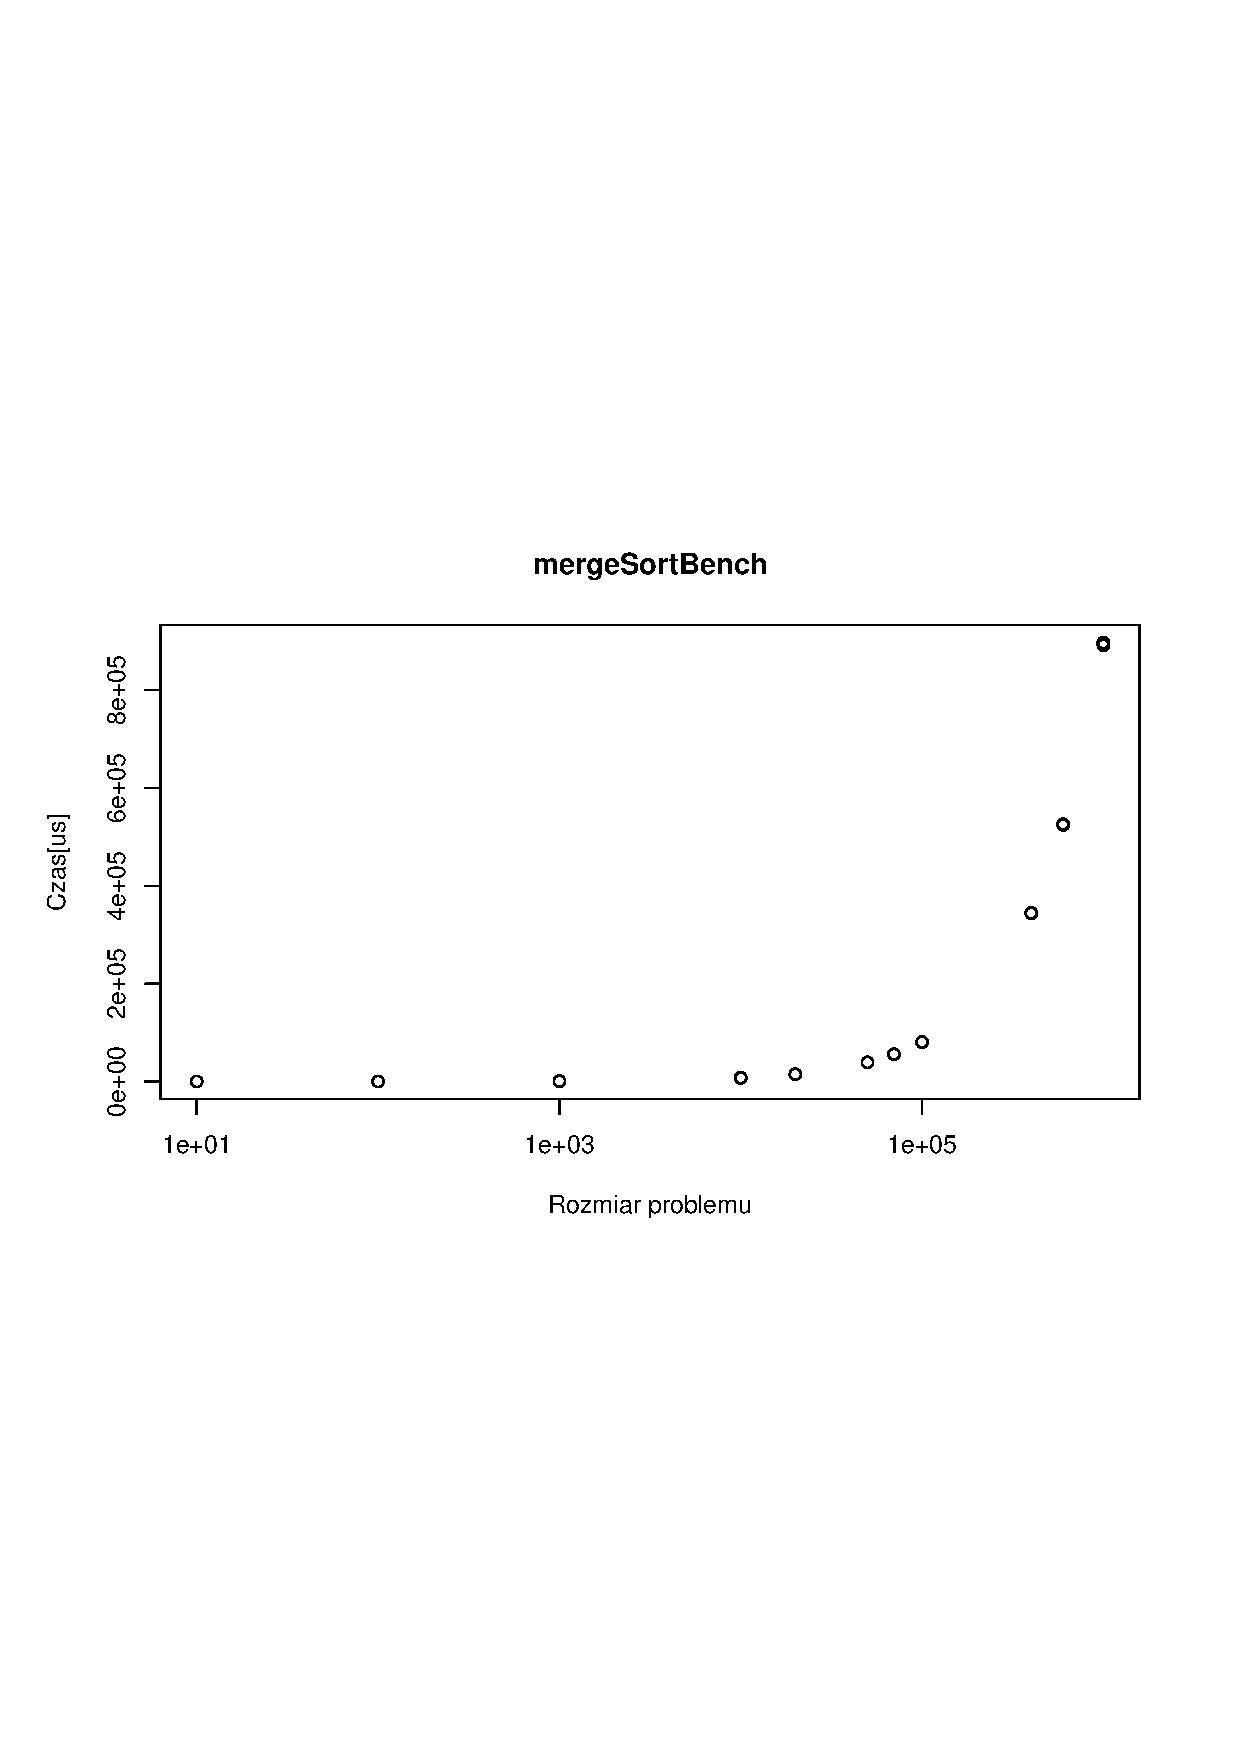
\includegraphics[width=0.7\linewidth]{./Wykresy/mergeSortBench}
\caption{Zależność czasu wykonania od rozmiaru problemu - Merge Sort}
\label{fig:mergeSortBench}
\end{figure}


\section{Wnioski i uwagi}

\begin{itemize}
	\item Aby pokazać złożoność algorytmów, w ostatnich trzech przypadkach użyłem
		skali logarytmicznej dla osi odciętych
	\item Widać, że quick sort jest bardzo wolny dla pesymistycznego przypadku
	\item Quick Sort nie był najszybszym algorytmem w tym teście nawet dla przypadku średniego,
	 przyczyną może być wybór piwota, który jest zawsze ostatnim elementem tablicy
	 \item Widać, że te trzy algorytmy mają złożoność $\mathcal{O}(\log_2 n)$, dla
	 sortowania szybkiego tyczy się to przypadku średniego
	 \item Widać, że w przypadku poprawionego algorytmu Quick Sort, złożoność obliczeniowa w
	 przypadku pesymistycznym znacznie się poprawiła. Można również zaobserwować, że punkty
	 dla tego samego rozmiaru nie są aż tak skupione. Jest to spowodowane losowaniem piwotu.
	\item Doszukałem się dwóch powodów, które mogą powodować, że Quick 
	Sort nie jest tak szybki. Metoda partition, którą oparłem na 
	algorytmie podanym w książce ,,Wprowadzenie do algorytmów'' 
	nie jest najszybsza, istnieją szybsze algorytmy podziału.
	Po drugie, powodem mogą być iteratory i narzut jaki ze sobą niosą.
\end{itemize}
\end{document}